\documentclass[11pt]{article}

% Input encoding
\usepackage[utf8]{inputenc}

% Geometry
\usepackage{geometry}
\geometry{margin=1in}
\setlength{\parskip}{1em} % Vertical space between paragraphs
\setlength{\parindent}{0pt} % Remove indentation

% Subliminal refinements towards typographical perfection
\usepackage[tracking=true]{microtype}

% Subtitle
\usepackage{titling}

% Good old Computer Modern
\usepackage{amsfonts}
\usepackage{amssymb}
\usepackage{bm}
\usepackage[T1]{fontenc}

% Mathematical typesetting
\usepackage{amsmath} % Base
\usepackage{amsthm} % Theorems
\usepackage{mathtools} % Tools to use with amsmath
\usepackage{xfrac} % Split-level fractions

% Generic symbols
\usepackage{textcomp}
\usepackage{gensymb}

% Plotting
\usepackage{tikz}            % Plots
\usepackage{tikz-3dplot}     % 3D plots
\usetikzlibrary{arrows.meta, positioning}

% Hyperlinks
\usepackage[
    colorlinks=true,
    linkcolor=blue,
    urlcolor=blue,
    citecolor=blue
]{hyperref}

% Custom packages
\usepackage{../common/my-headings}
\usepackage{../common/my-list-control}
\usepackage{../common/my-math-macros}
\usepackage{../common/my-matrix-control}
\usepackage{../common/my-subtitle}
\usepackage{../common/my-theorem-envs}


\title{Mathematics for Machine Learning}
\subtitle{Exercises 3: Analytic geometry}
\author{}
\date{}

\begin{document}

\maketitle

\begin{enumerate}

    \item[3.1] Show that $\inner{\cdot}{\cdot}$, defined for all $\x = [x_1, x_2]^\top \in \R^2$ and
          $\y = [y_1, y_2]^\top \in \R^2$ by
          \[
              \inner{\x}{\y} = x_1 y_1 - (x_1 y_2 + x_2 y_1) + 2 x_2 y_2,
          \]
          is an inner product.

          \vspace{1em}

          An inner product must be:

          \subsubsubsection{Symmetric}
          \[
              \forall \x, \y \in \R^2 : \inner{\x}{\y} = \inner{\y}{\x}
          \]

          \subsubsubsection{Bilinear}
          \[
              \forall \x, \y, \z \in \R^2, \;
              \forall \lambda, \phi \in \R :
              \begin{cases}
                  \inner{ \lambda \x + \phi \y }{ \z } = \lambda \inner{\x}{\z} + \phi \inner{\y}{\z}, \\
                  \inner{ \x }{ \lambda \y + \phi \z } = \lambda \inner{\x}{\y} + \phi \inner{\x}{\z}. \\
              \end{cases}
          \]

          \subsubsubsection{Positive definite}
          \[
              \forall \x \in \R^2 \setminus \set{\vect{0}} :
              \inner{\x}{\x} > 0,
              \qquad
              \inner{\vect{0}}{\vect{0}} = 0
          \]

          That the given $\inner{\cdot}{\cdot}$ is symmetric is obvious.  For bilinearity, consider that fixing
          one argument while holding the other constant, there are only linear terms in the components of each (no
          quadratic terms).  For positive definiteness, consider
          \[
              \begin{aligned}
                  \inner{\x}{\x} & = x_1^2 - 2 x_1 x_2 + 2 x_2^2 \\
                                 & = (x_1 - x_2)^2 + x_2^2
              \end{aligned}
          \]
          which is always positive for non-zero $x_1, x_2$, and $\inner{\vect{0}}{\vect{0}} = 0$, as required.

          This inner product may be represented with the following symmetric positive definite matrix:
          \[
              \begin{aligned}
                  \mat{A} :=
                  \begin{bmatrix}
                      \begin{array}{@{}i{3}i{3}@{\;\;}}
                          1  & -1 \\
                          -1 & 2  \\
                      \end{array}
                  \end{bmatrix}
                  \qquad
                  \inner{\x}{\y} = \x^\top \mat{A} \y
              \end{aligned}
          \]

          \pagebreak

    \item[3.2] Consider $\R^2$ with $\inner{\cdot}{\cdot}$ defined for all $\x, \y$ in $\R^2$ as
          \[
              \inner{\x}{\y} = \x^\top
              \underbrace{
                  \begin{bmatrix}
                      2 & 0 \\
                      1 & 2 \\
                  \end{bmatrix}
              }_{
              \mat{A} :=
              }
              \y
          \]
          Is $\inner{\cdot}{\cdot}$ an inner product?

          \vspace{1em}

          No.  An inner product may only be defined by a symmetric positive definite matrix.  Since $\mat{A}$ is
          not symmetric, $\inner{\cdot}{\cdot}$ is not symmetric in its arguments.

    \item[3.3] Compute the distance between
          \[
              \x = \begin{bmatrix}
                  \begin{array}{i{1}}
                      1 \\ 2 \\ 3
                  \end{array}
              \end{bmatrix}
              \qquad
              \y = \begin{bmatrix}
                  \begin{array}{@{}i{3}@{\,}}
                      -1 \\ -1 \\ 0
                  \end{array}
              \end{bmatrix}
          \]

          \begin{enumerate}
              \item[a.] Using $\inner{\x}{\y} = \x^\top \y$
                    \[
                        \x - \y = \begin{bmatrix}
                            \begin{array}{i{1}}
                                2 \\ 3 \\ 3
                            \end{array}
                        \end{bmatrix}
                        \qquad
                        \begin{aligned}
                            d(\x, \y) & = \norm{ \x - \y }                    \\
                                      & = \sqrt{\inner{ \x - \y }{ \x - \y }} \\
                                      & = \sqrt{22}                           \\
                                      & \approx 4.69
                        \end{aligned}
                    \]

              \item[b.] Using $\inner{\x}{\y} = \x^\top \mat{A} \y, \quad \mat{A} :=
                        \begin{bmatrix}
                            \begin{array}{@{\;}i{1}i{3}i{3}@{\;}}
                                2 & 1  & 0  \\
                                1 & 3  & -1 \\
                                0 & -1 & 2  \\
                            \end{array}
                        \end{bmatrix}
                    $
                    \[
                        \mat{A} (\vect{x} - \vect{y}) =
                        \begin{bmatrix}
                            \begin{array}{i{1}}
                                7 \\ 8 \\ 3
                            \end{array}
                        \end{bmatrix}
                        \qquad
                        (\vect{x} - \vect{y})^\top \mat{A} (\vect{x} - \vect{y}) = 47
                        \qquad
                        d(\x, \y) = \sqrt{47} \approx 6.86
                    \]

          \end{enumerate}

    \item[3.4] Compute the angle between
          \[
              \x = \begin{bmatrix}
                  \begin{array}{@{\;}i{1}@{\;}}
                      1 \\ 2
                  \end{array}
              \end{bmatrix}
              \qquad
              \y = \begin{bmatrix}
                  \begin{array}{@{}i{3}@{\,}}
                      -1 \\ -1
                  \end{array}
              \end{bmatrix}
          \]

          \begin{enumerate}
              \item[a.] Using $\inner{\x}{\y} = \x^\top \y$
                    \[
                        \cos \theta
                        = \frac{ \inner{\x}{\y} }{ \norm{\x} \norm{\y} }
                        \qquad
                        \inner{\x}{\y} = -3
                        \qquad
                        \norm{\x} = \sqrt{5}
                        \qquad
                        \norm{\y} = \sqrt{2}
                        \qquad
                        \theta \approx 161.6\degree
                    \]

              \item[b.] Using $\inner{\x}{\y} = \x^\top \mat{B} \y, \quad \mat{B} :=
                        \begin{bmatrix}
                            \begin{array}{@{\;}i{1}i{1}@{\;}}
                                2 & 1 \\
                                1 & 3 \\
                            \end{array}
                        \end{bmatrix}
                    $
                    \[
                        \mat{B} \x =
                        \begin{bmatrix}
                            \begin{array}{@{\,}i{1}@{\,}}
                                4 \\ 7
                            \end{array}
                        \end{bmatrix}
                        \quad
                        \mat{B} \y =
                        \begin{bmatrix}
                            \begin{array}{@{}i{3}@{\,}}
                                -3 \\ -4
                            \end{array}
                        \end{bmatrix}
                        \quad \;\;
                        \inner{\x}{\y} = -11
                        \quad \;\;
                        \norm{\x} = \sqrt{18}
                        \quad \;\;
                        \norm{\y} = \sqrt{7}
                        \quad \;\;
                        \theta \approx 168.5\degree
                    \]
          \end{enumerate}

    \item[3.5] Consider the Euclidean vector space $\R^5$ with the dot product. A subspace $U \subseteq \R^5$ and
          $\x \in \R^5$ are given by
          \[
              U = \Span \args{
                  \begin{bmatrix}
                      \begin{array}{@{}i{3}@{\;}}
                          0 \\ -1 \\ 2 \\ 0 \\ 2
                      \end{array}
                  \end{bmatrix}
                  \! ,
                  \begin{bmatrix}
                      \begin{array}{@{}i{3}@{\;}}
                          1 \\ -3 \\ 1 \\ -1 \\ 2
                      \end{array}
                  \end{bmatrix}
                  \! ,
                  \begin{bmatrix}
                      \begin{array}{@{}i{3}@{\;}}
                          -3 \\ 4 \\ 1 \\ 2 \\ 1
                      \end{array}
                  \end{bmatrix}
                  \! ,
                  \begin{bmatrix}
                      \begin{array}{@{}i{3}@{\;}}
                          -1 \\ -3 \\ 5 \\ 0 \\ 7
                      \end{array}
                  \end{bmatrix}
              }
              \qquad
              \x =
              \begin{bmatrix}
                  \begin{array}{@{}i{3}@{\;}}
                      -1 \\ -9 \\ -1 \\ 4 \\ 1
                  \end{array}
              \end{bmatrix}
          \]

          \begin{enumerate}
              \item[a.] Determine the orthogonal projection $\pi_U(\x)$ of $\x$ onto $U$.
              \item[b.] Determine the distance $d(\x, U)$.

                    \vspace{1em}

                    Let $\mat{B} = [ \vect{b}_1 \; \vect{b}_2 \; \vect{b}_3 \; \vect{b}_4  ]$, where the respective
                    $\vect{b}_i$ are the vectors in the span of $U$ as above, and let $\vect{\lambda} = [ \lambda_1 \;
                        \lambda_2 \; \lambda_3 \; \lambda_4 ]^\top$, such that $\pi_U(\x) = \mat{B}\vect{\lambda}$, where
                    $\vect{\lambda}$ gives the coordinates of the projection of $\x$ onto $U$, relative to the ordered
                    basis of $U$.

                    The residual, $\x - \mat{B} \vect{\lambda}$, must be orthogonal to each basis vector:
                    \[
                        \begin{aligned}
                            \inner{\vect{b}_1}{\x - \mat{B}\vect{\lambda}} & = 0 \\ & \shortvdotswithin{=}
                            \inner{\vect{b}_4}{\x - \mat{B}\vect{\lambda}} & = 0 \\
                        \end{aligned}
                    \]
                    which, given bilinearity and our use of the standard dot product, is equivalently:
                    \[
                        \begin{aligned}
                            \inner{\vect{b}_1}{\mat{B}\vect{\lambda}} & = \inner{\vect{b}_1}{\x} \\ & \shortvdotswithin{=}
                            \inner{\vect{b}_4}{\mat{B}\vect{\lambda}} & = \inner{\vect{b}_4}{\x} \\
                        \end{aligned}
                        \quad
                        \iff
                        \quad
                        \begin{aligned}
                            \vect{b}_1^\top \mat{B}\vect{\lambda} & = \vect{b}_1^\top \x \\ & \shortvdotswithin{=}
                            \vect{b}_4^\top \mat{B}\vect{\lambda} & = \vect{b}_4^\top \x \\
                        \end{aligned}
                        \quad
                        \iff
                        \quad
                        \mat{B}^\top \mat{B} \vect{\lambda} = \mat{B}^\top \x \\ [2pt]
                    \]

                    Note, we find $\mat{B}$ is rank 3 — its columns are linearly dependent.  Consequently, its Gram
                    matrix ($\mat{B}^\top \mat{B}$) is singular.  Below, we proceed to find $\vect{\lambda}'$ with
                    Gaussian elimination, but note it may instead be computed directly by inverting the Gram matrix in
                    the expression on the right above — though only if the Gram matrix is invertible.

                    So, discarding $\vect{b}_4$ and $\lambda_4$, let $\mat{B}' = [\vect{b}_1  \; \vect{b}_2 \;
                        \vect{b}_3]$, eliminate $[ \, \mat{B}'^\top \mat{B} \, \mid \, \mat{B}'^\top \x \, ]
                        \rightsquigarrow [ \; \mat{I} \, \mid \, \vect{\lambda}' \; ]$, and finally find $\pi_U(\x) = \mat{B}
                        \vect{\lambda}'$, and the corresponding residual:
                    \[
                        \begin{aligned}
                            \begin{bmatrix}
                                \begin{array}{@{}i{3}i{4}i{4}|i{4}@{\;}}
                                    9 & 9   & 0   & 9   \\
                                    9 & 16  & -14 & 23  \\
                                    0 & -14 & 31  & -25 \\
                                \end{array}
                            \end{bmatrix}
                             & \rightsquigarrow
                            \begin{bmatrix}
                                \begin{array}{@{}i{2}i{4}i{4}|i{4}@{\;}}
                                    1 & 1   & 0   & 1   \\
                                    0 & 7   & -14 & 14  \\
                                    0 & -14 & 31  & -25 \\
                                \end{array}
                            \end{bmatrix}
                            \\
                             & \rightsquigarrow
                            \begin{bmatrix}
                                \begin{array}{@{}i{2}i{4}i{4}|i{4}@{\;}}
                                    1 & 1 & 0  & 1 \\
                                    0 & 1 & -2 & 2 \\
                                    0 & 0 & 3  & 3 \\
                                \end{array}
                            \end{bmatrix}
                            \\
                             & \rightsquigarrow
                            \begin{bmatrix}
                                \begin{array}{@{}i{2}i{4}i{4}|i{4}@{\;}}
                                    1 & 0 & 0 & -3 \\
                                    0 & 1 & 0 & 4  \\
                                    0 & 0 & 1 & 1  \\
                                \end{array}
                            \end{bmatrix}
                        \end{aligned}
                        \qquad
                        \begin{aligned}
                            \pi_U(\x)      & =
                            \begin{bmatrix}
                                \begin{array}{@{}i{3}@{\;}}
                                    1 \\ -5  \\ -1  \\ -2 \\ 3
                                \end{array}
                            \end{bmatrix}
                            \\
                            \x - \pi_U(\x) & =
                            \begin{bmatrix}
                                \begin{array}{@{}i{3}@{\;}}
                                    -2 \\ -4  \\ 0 \\ 6 \\ -2
                                \end{array}
                            \end{bmatrix}
                        \end{aligned}
                    \]
                    Compute the distance, $d(\x, U) = \norm{\x - \pi_U(\x)} = \sqrt{60} = 2 \sqrt{15} \approx 7.75$.

                    \pagebreak
          \end{enumerate}

    \item[3.6] Consider $\R^3$ with the inner product $\inner{\x}{\y} := \x^\top \mat{A} \y$, where
          \[
              \mat{A} :=
              \begin{bmatrix}
                  \begin{array}{@{}i{2}i{3}i{3}@{\;}}
                      2 & 1  & 0  \\
                      1 & 2  & -1 \\
                      0 & -1 & 2  \\
                  \end{array}
              \end{bmatrix}
          \]
          Furthermore, define $\vect{e}_1, \vect{e}_2, \vect{e}_3$ to be the standard / canonical basis in
          $\R^3$.

          \begin{enumerate}
              \item[a.] Determine the orthogonal projection $\pi_U(\vect{e}_2)$ of $\vect{e}_2$ onto
                    \[
                        U = \Span \args{\vect{e}_1, \vect{e}_3}.
                    \]

              \item[b.] Compute the distance $d(\vect{e}_2, U)$.

              \item[c.] Draw the scenario, standard basis vectors and $\pi_U(\vect{e}_2)$.
          \end{enumerate}

          \vspace{1em}

          Let $\mat{B} = [\vect{e}_1 \; \vect{e}_3]$, and let $\vect{\lambda} = [\lambda_1 \; \lambda_2]^\top$
          be the coordinates of $\pi_U(\vect{e}_2)$ in the ordered basis of $U$, such that
          $\pi_U(\vect{e}_2) = \mat{B} \vect{\lambda}$.  Then
          \[
              \begin{aligned}
                  \inner{ \vect{e}_1 }{ \vect{e}_2 - \mat{B} \vect{\lambda} } = 0 \\
                  \inner{ \vect{e}_3 }{ \vect{e}_2 - \mat{B} \vect{\lambda} } = 0 \\
              \end{aligned}
              \quad
              \iff
              \quad
              \begin{aligned}
                  \vect{e}_1^\top \mat{A} \vect{e}_2 = \vect{e}_1^\top \mat{A} \mat{B} \vect{\lambda} \\
                  \vect{e}_3^\top \mat{A} \vect{e}_2 = \vect{e}_3^\top \mat{A} \mat{B} \vect{\lambda} \\
              \end{aligned}
              \quad
              \iff
              \quad
              \mat{B}^\top \mat{A} \vect{e}_2 = \mat{B}^\top \mat{A} \mat{B} \vect{\lambda}
          \]
          Computing
          \[
              \mat{B}^\top \mat{A} \vect{e}_2 =
              \mat{B}^\top \!
              \begin{bmatrix}
                  \begin{array}{@{}i{3}@{\;}}
                      1 \\ 2 \\ -1
                  \end{array}
              \end{bmatrix}
              =
              \begin{bmatrix}
                  \begin{array}{@{}i{3}@{\;}}
                      1 \\ -1
                  \end{array}
              \end{bmatrix}
              \qquad
              \mat{B}^\top \mat{A} \mat{B} =
              \mat{B}^\top
              \begin{bmatrix}
                  \begin{array}{@{}i{2}i{3}@{\;}}
                      2 & 0  \\
                      1 & -1 \\
                      0 & 2  \\
                  \end{array}
              \end{bmatrix}
              =
              \begin{bmatrix}
                  \begin{array}{@{\;}i{1}i{1}@{\;}}
                      2 & 0 \\
                      0 & 2 \\
                  \end{array}
              \end{bmatrix}
          \]
          \[
              \vect{\lambda} =
              \begin{bmatrix}
                  \begin{array}{@{\,}r}
                      \sfrac{1}{2} \\ -\sfrac{1}{2}
                  \end{array}
              \end{bmatrix}
              \qquad
              \pi_U(\vect{e}_2) =
              \begin{bmatrix}
                  \begin{array}{@{\,}r}
                      \sfrac{1}{2} \\ 0 \\ -\sfrac{1}{2}
                  \end{array}
              \end{bmatrix}
              \qquad
              \vect{e}_2 - \pi_U(\vect{e}_2) =
              \begin{bmatrix}
                  \begin{array}{@{\,}r}
                      -\sfrac{1}{2} \\ 1 \\ \sfrac{1}{2}
                  \end{array}
              \end{bmatrix}
          \]
          Finally,
          \[
              \begin{aligned}
                  d(\vect{e}_2, U) & = \norm{ \vect{e}_2 - \pi_U(\vect{e}_2) }                                                   \\
                                   & = \sqrt{( \vect{e}_2 - \pi_U(\vect{e}_2) )^\top \mat{A} ( \vect{e}_2 - \pi_U(\vect{e}_2) )} \\
                                   & = \sqrt{
                      \begin{bmatrix}
                          \begin{array}{@{\,}r}
                              -\sfrac{1}{2} \\ 1 \\ \sfrac{1}{2}
                          \end{array}
                      \end{bmatrix}^\top
                      \begin{bmatrix}
                          \begin{array}{c}
                              0 \\ 1 \\ 0
                          \end{array}
                      \end{bmatrix}
                  }
                  \\
                                   & = 1.
              \end{aligned}
          \]

          \vspace{1em}
          \makebox[\linewidth][c]{%
              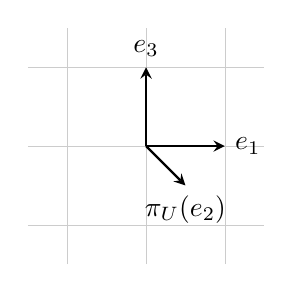
\begin{tikzpicture}[>=stealth]
                  % Grid
                  \draw[help lines, gray!40] (-1.5, -1.5) grid (1.5, 1.5);

                  % U basis
                  \draw[->, thick, black] (0, 0) -- (1, 0) node[right] {$\vect{e}_1$};
                  \draw[->, thick, black] (0, 0) -- (0, 1) node[above] {$\vect{e}_3$};

                  % Projection
                  \draw[->, thick, black] (0, 0) -- (0.5, -0.5) node[below] {$\pi_U(\vect{e}_2)$};
              \end{tikzpicture}
          }

          \pagebreak

    \item[3.7] Let $V$ be a vector space and $\pi$ an endomorphism of $V$.

          \begin{enumerate}
              \item[a.] Prove that $\pi$ is a projection if and only if $\id_V - \pi$ is a projection, where $\id_V$
                    is the identity endomorphism on $V$.

                    \begin{proof}
                        Define $\rho = \id_V - \pi$.  Then
                        \[
                            \rho^2 = \id_V - 2 \pi + \pi^2.
                        \]
                        \[
                            \rho^2 = \rho
                            \begin{aligned}
                                 & \quad \iff \quad
                                \id_V - 2 \pi + \pi^2 = \id_V - \pi \\
                                 & \quad \iff \quad
                                \pi^2 = \pi                         \\
                            \end{aligned}
                        \]
                    \end{proof}

              \item[b.] Assume now that $\pi$ is a projection.  Calculate $\Img(\id_V - \pi)$ and $\ker(\id_V
                        - \pi)$ as a function of $\Img(\pi)$ and $\ker(\pi)$.
                    \[
                        \Img(\id_V - \pi) = \ker(\pi)
                    \]
                    \begin{proof}
                        Let $\vect{v} \in \Img(\id_V - \pi)$, let $\vect{u} \in V$ be a preimage of $\vect{v}$ under
                        $\id_V - \pi$, and consider:
                        \[
                            \begin{aligned}
                                \vect{v}      & = (\id_V - \pi)(\vect{u})                   \\
                                              & = \vect{u} - \pi(\vect{u}),                 \\
                                \pi(\vect{v}) & = \pi(\vect{u}) - \pi(\pi(\vect{u}))        \\
                                              & = \pi(\vect{u}) - \pi(\vect{u})             \\
                                              & = \vect{0} \implies \vect{v} \in \ker(\pi).
                            \end{aligned}
                        \]
                        Then let $\vect{w} \in \ker(\pi)$, and consider:
                        \[
                            \begin{aligned}
                                \pi(\vect{w})           & = \vect{0},                                         \\
                                (\id_V - \pi)(\vect{w}) & = \vect{w} - \pi(\vect{w})                          \\
                                                        & = \vect{w} \implies \vect{w} \in \Img(\id_V - \pi).
                            \end{aligned}
                        \]
                    \end{proof}

                    \[
                        \ker(\id_V - \pi) = \Img(\pi)
                    \]
                    \begin{proof}
                        Let $\vect{w} \in \ker(\id_V - \pi)$, and consider:
                        \[
                            \begin{alignedat}{2}
                                         &  & (\id_V - \pi)(\vect{w}) & = \vect{w} - \pi(\vect{w}) = \vect{0} \\
                                \iff     &  & \pi(\vect{w})           & = \vect{w}                            \\
                                \implies &  & \vect{w} \in \Img(\pi)  & .
                            \end{alignedat}
                        \]
                        Then let $\vect{v} \in \Img(\pi)$, let $\vect{u} \in V$ be a preimage of $\vect{v}$ under $\id_V - \pi$, and consider:
                        \[
                            \begin{aligned}
                                \pi(\vect{u})           & = \vect{v},                                         \\
                                (\id_V - \pi)(\vect{v}) & = \vect{v} - \pi(\vect{v})                          \\
                                                        & = \pi(\vect{u}) - \pi(\pi(\vect{u}))                \\
                                                        & = \pi(\vect{u}) - \pi(\vect{u})                     \\
                                                        & = \vect{0} \implies \vect{v} \in \ker(\id_V - \pi).
                            \end{aligned}
                        \]
                    \end{proof}
          \end{enumerate}

    \item[3.8] Using the Gram-Schmidt method, turn the basis $B = (\vect{b}_1, \vect{b}_2)$ of a two-dimensional
          subspace $U \subseteq \R^3$ into an orthonormal basis, $C = (\vect{c}_1, \vect{c}_2)$ of $U$, where
          \[
              \vect{b}_1 :=
              \begin{bmatrix}
                  \begin{array}{@{\;}i{1}@{\;}}
                      1 \\ 1 \\ 1
                  \end{array}
              \end{bmatrix} \! ,
              \qquad
              \vect{b}_2 :=
              \begin{bmatrix}
                  \begin{array}{@{}i{3}@{\;}}
                      -1 \\ 2 \\ 0
                  \end{array}
              \end{bmatrix} \! .
          \]
          Let $\vect{u}_1 = \vect{b}_1$.  Then let $\vect{u}_2 = \vect{b}_2 - \pi_{\vect{u}_1}\!(\vect{b}_2)$, where
          $\pi_{\vect{u}_1}$ is the projection operator onto the one-dimensional subspace spanned by $\vect{u}_1$.
          Assuming the standard dot product,
          \[
              \pi_{\vect{u}_1}(\vect{b}_2)
              = \frac{ \vect{u}_1 \vect{u}_1^\top }{ \norm{\vect{u}_1}^2 } \vect{b}_2
              = \frac{1}{3}
              \begin{bmatrix}
                  \begin{array}{@{\;}i{1}i{1}i{1}@{\;}}
                      1 & 1 & 1 \\
                      1 & 1 & 1 \\
                      1 & 1 & 1 \\
                  \end{array}
              \end{bmatrix}
              \begin{bmatrix}
                  \begin{array}{@{}i{3}@{\;}}
                      -1 \\ 2 \\ 0
                  \end{array}
              \end{bmatrix}
              =
              \frac{1}{3} \!
              \begin{bmatrix}
                  \begin{array}{@{\;}i{1}@{\;}}
                      1 \\ 1 \\ 1
                  \end{array}
              \end{bmatrix} \! ,
              \qquad
              \vect{u}_2 =
              \frac{1}{3} \!
              \begin{bmatrix}
                  \begin{array}{@{}i{3}@{\;}}
                      -4 \\ 5  \\ -1
                  \end{array}
              \end{bmatrix} \! .
          \]
          Normalizing each of $\vect{u}_1$ and $\vect{u}_2$, we define our orthonormal basis vectors to be:
          \[
              \vect{c}_1
              := \frac{ \vect{u}_1 }{ \norm {\vect{u}_1} }
              = \frac{\sqrt{3}}{3} \!
              \begin{bmatrix}
                  \begin{array}{@{\;}i{1}@{\;}}
                      1 \\ 1 \\ 1
                  \end{array}
              \end{bmatrix} \! ,
              \qquad
              \vect{c}_2
              := \frac{ \vect{u}_2 }{ \norm {\vect{u}_2} }
              = \frac{\sqrt{42}}{42} \!
              \begin{bmatrix}
                  \begin{array}{@{}i{3}@{\;}}
                      -4 \\ 5 \\ -1
                  \end{array}
              \end{bmatrix} \! .
          \]

    \item[3.9] Let $n \in \N$ and let $a_1, \ldots, a_n > 0$ be $n$ positive real numbers so that $\sum_{i = 1}^n a_i =
              1$.  Use the Cauchy-Schwarz inequality to show that:
          \[
              \text{a.} \; \sum_{i = 1}^n a_i^2 \geq \frac{1}{n}
              \qquad \qquad
              \text{b.} \; \sum_{i = 1}^n \frac{1}{a_i} \geq n^2
          \]

          \[
              \lim_{k \rightarrow \infty} \left( \frac{(k - (n - 1))^2}{k^2} + \sum_{i=1}^{n-1} \frac{1}{k^2} \right)
              = \lim_{k \rightarrow \infty} \left( \frac{(k - (n - 1))^2}{k^2} + \frac{n-1}{k^2} \right) = 1.
          \]

          \begin{enumerate}
              \item[a.] Let $\x = [ a_1 \; \cdots \; a_n ]^\top$ and let $\y = [ 1 \; \cdots \; 1 ]^\top \in \R^n$.
                    Then, using the standard inner product:
                    \[
                        \norm{\x}^2
                        = \x^\top \x
                        = \sum_{i = 1}^n a_i^2
                        \qquad
                        \norm{\y}^2
                        = \y^\top \y
                        = \sum_{i=1}^n 1 = n
                    \]
                    \[
                        \inner{\x}{\y}
                        = \x^\top \y
                        = \sum_{i=1}^n a_i = 1
                    \]
                    Cauchy-Schwarz:
                    \[
                        \begin{aligned}
                                       & \abs{\inner{\x}{\y}} \leq \norm{\x} \norm{\y} \\
                            \iff \quad & \inner{\x}{\y}^2 \leq \norm{\x}^2 \norm{\y}^2 \\
                        \end{aligned}
                    \]
                    Substituting:
                    \[
                        1 \leq n \sum_{i=1}^n a_i^2
                        \quad \iff \quad
                        \frac{1}{n} \leq \sum_{i=1}^n a_i^2.
                    \]

                    \pagebreak

              \item[b.] Let $\x = \left [ \frac{1}{\sqrt{a_1}} \; \cdots \; \frac{1}{\sqrt{a_n}} \right ]^\top$ and let
                    $\y = \left [ \sqrt{a_1} \; \cdots \; \sqrt{a_n} \right ]^\top$. Then:
                    \[
                        \norm{\x}^2
                        = \x^\top \x
                        = \sum_{i=1}^n \left ( \frac{1}{\sqrt{a_i}} \right )^2
                        = \sum_{i=1}^n \frac{1}{a_i}
                        \qquad
                        \norm{\y}^2
                        = \y^\top \y
                        = \sum_{i=1}^n \left ( \sqrt{a_i} \right )^2
                        = \sum_{i=1}^n a_i = 1
                    \]
                    \[
                        \inner{\x}{\y}
                        = \x^\top \y
                        = \sum_{i=1}^n \frac{\left ( \sqrt{a_i} \right )^2}{a_i} = \sum_{i=1}^n 1 = n.
                    \]
                    Substituting:
                    \[
                        n^2
                        \leq \sum_{i=1}^n \frac{1}{a_i}.
                    \]
          \end{enumerate}

    \item[3.10] Rotate the following vectors by 30\degree:
          \[
              \x_1 :=
              \begin{bmatrix}
                  \begin{array}{@{\;}i{1}@{\;}}
                      2 \\ 3
                  \end{array}
              \end{bmatrix}
              \qquad
              \x_2 :=
              \begin{bmatrix}
                  \begin{array}{@{}i{3}@{\;}}
                      0 \\ -1
                  \end{array}
              \end{bmatrix}
          \]
          \[
              \mat{R}_{30\degree}
              =
              \begin{bmatrix}
                  \begin{array}{rr}
                      \cos \sfrac{\pi}{6} & -\sin \sfrac{\pi}{6} \\
                      \sin \sfrac{\pi}{6} & \cos \sfrac{\pi}{6}  \\
                  \end{array}
              \end{bmatrix}
              =
              \tfrac{1}{2}
              \begin{bmatrix}
                  \begin{array}{cc}
                      \sqrt{3} & -1       \\
                      1        & \sqrt{3} \\
                  \end{array}
              \end{bmatrix}
          \]
          \vspace{0.5em}
          \[
              \mat{R}_{30\degree} \x_1
              =
              \tfrac{1}{2}
              \begin{bmatrix}
                  \begin{array}{c}
                      2 \sqrt{3} - 3 \\
                      3 \sqrt{3} + 2 \\
                  \end{array}
              \end{bmatrix}
              \approx
              \begin{bmatrix}
                  \begin{array}{c}
                      0.23 \\
                      3.60 \\
                  \end{array}
              \end{bmatrix}
              \qquad
              \mat{R}_{30\degree} \x_2
              =
              \tfrac{1}{2}
              \begin{bmatrix}
                  \begin{array}{c}
                      1         \\
                      -\sqrt{3} \\
                  \end{array}
              \end{bmatrix}
              \approx
              \begin{bmatrix}
                  \begin{array}{@{\,}r}
                      0.50  \\
                      -0.87 \\
                  \end{array}
              \end{bmatrix}
          \]

          \vspace{1em}
          \makebox[\linewidth][c]{%
              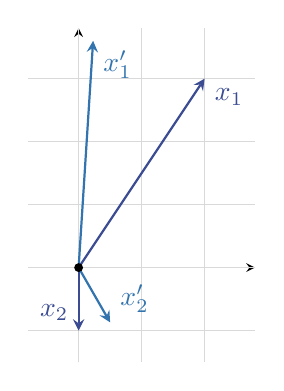
\begin{tikzpicture}[
                      scale=0.8,
                      >=stealth,
                  ]
                  \tikzset{
                      vec_p/.style = {thick, cyan!20!blue!80!black},
                      vec_i/.style = {thick, cyan!60!blue!80!black},
                  }

                  % Axes
                  \draw[->] (-0.8,0) -- (2.8,0);
                  \draw[->] (0,-1.5) -- (0,3.8);

                  % Grid
                  \draw[help lines, gray!30] (-0.8,-1.5) grid (2.8,3.8);

                  % New vectors x1', x2'
                  \draw[->, vec_i] (0,0) -- (0.23,3.60) node[below right] {$\vect{x}'_1$};
                  \draw[->, vec_i] (0,0) -- (0.5,-0.87) node[above right] {$\vect{x}'_2$};

                  % Original vectors x1, x2
                  \draw[->, vec_p] (0,0) -- (2,3) node[below right] {$\vect{x}_1$};
                  \draw[->, vec_p] (0,0) -- (0,-1) node[above left] {$\vect{x}_2$};

                  % Origin
                  \fill (0,0) circle (2pt);

              \end{tikzpicture}
          }

\end{enumerate}

\end{document}